\documentclass[12pt]{article}
\usepackage[vietnamese]{babel}
\usepackage{graphicx}
\usepackage{listings}
\title{IT003: Cấu trúc dữ liệu và giải thuật}
\author{Châu Nguyên Khang - MTIC2024}
\begin{document}
\maketitle
\par
Đây là đề cương tự là của môn cấu trúc dữ liệu và giải thuật dựa trên các slide của 
Trường Đại học Công nghệ thông tin và các trang web trên Internet. Mục đích tài liệu là sử dụng cho vấn đề học tập 
trên trường, không sử dụng với bất kì mục đích thương mại nào.
\newpage
\section{Chương 1: Thuật toán sắp xếp}
\subsection{Thuật toán sắp xếp chọn trực tiếp (Insertion Sort)}
\begingroup
    a)\textbf{\underline{Mô tả bài toán:}}
    
    \textbf{Input}: Cho một dãy a có n phần tử chưa được sắp xếp.

    \textbf{Output}: Một dãy a có n phần tử đã được sắp xếp.
    \newline
\endgroup
\begingroup
    b)\textbf{\underline{Ý tưởng thuật toán:}}

    \textbf{Bước 1:} Ta bắt đầu bằng phần tử đầu tiên trong mảng. Vì phần tử đầu tiên
    chúng ta xem như là đã sắp xếp rồi.

    \textbf{Bước 2:} Ta kiểm tra xem phần tử thứ hai có nhỏ hơn phần tử thứ nhất không.
    Nếu có đổi chỗ phần tử thứ hai với phần tử thứ nhất.

    \textbf{Bước 3:} Ta chuyển sang phần tử thứ ba và so sánh với phần tử thứ nhất và
    phần tử thứ hai và đặt vào đúng vị trí.

    \textbf{Bước 4:} Lặp lại các bước trên cho đến khi mảng được sắp xếp xong.
\endgroup
\begin{figure}
    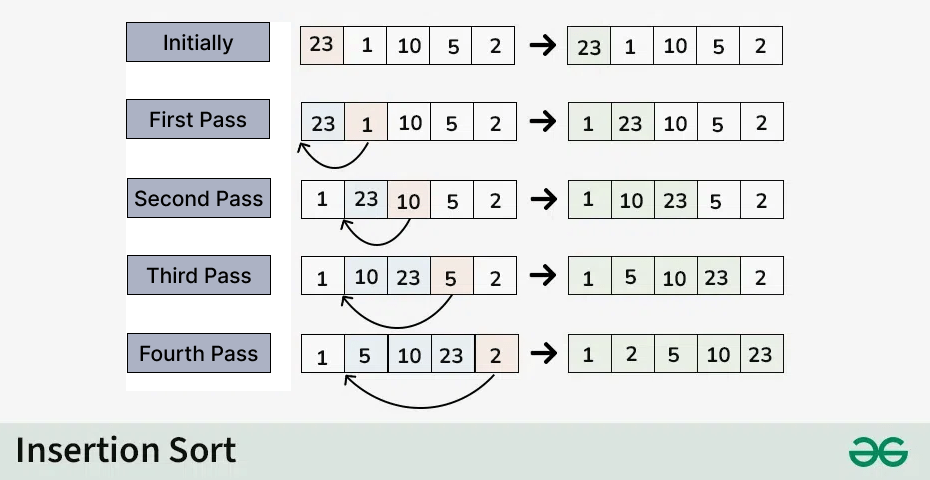
\includegraphics[width=12cm]{Insertion-sorting.jpg}
\end{figure}
\begin{lstlisting}[language = C++]
    #include <bits/stdc++.h>
    using namespace std;
    void Insertion_sort(vector <int> &a,int n){
    for (int i = 1; i < n; i++)
    {
        int key = a[i];
        int j = i - 1;
        while (j >= 0 && a[j] > key){
            a[j+1] = a[j];
            j--;
        }
        a[j+1] = key;
    }
}
int main(){
    freopen("test.inp","r",stdin);
    freopen("test.out","w",stdout);
    int n;
    cin >> n;
    vector <int> a;
    for (int i = 0; i < n; i++)
    {
        int x;
        cin >> x;
        a.push_back(x);
    }
    Insertion_sort(a,n);
    for (auto x : a){
        cout << x << " ";
    }
}
\end{lstlisting}
\end{document}